\chapter{CONCLUSION AND FUTURE WORK}
\label{chp:conclusion}

% Specific objective a) 

The reported accuracy results on the datasets exhibit significant inconsistency in the body of literature, aligning with the initial concern highlighted by \textcite{Ho2020} that "high accuracy does not imply reproducibility". The three benchmark datasets exhibit notable distinctions, despite originating from the same source repository (Freesound), they differ significantly in terms of sample duration and sound quality. ESC-10 and BDLib2 showcase cleaner signals predominantly focused on foreground sounds, whereas BDLib2 suffers from a lack of sample representativeness. Conversely, \gls{us8k} presents a mixture of background and foreground sounds and boasts a much larger sample size compared to both ESC-10 and BDLib2. One could posit a hypothesis that ESC-10 would achieve the highest accuracy rates, followed by BDLib2 and \gls{us8k}, in line with some findings in the literature, either using classical machine learning techniques such as \cite{Silva2019} and \cite{Bountourakis2019} or \gls{cnn} 1D such as \cite{Vandendriessche2021}, notably, these authors followed strictly the dataset specifications regarding k-fold cross-validation. Others like \cite{Lhoest2021} and \cite{Luz2021} achieved remarkably high accuracy rates for \gls{us8k} using Random Forest and \gls{k-nn}, respectively 94,2\% and 93,2\%), however, they didn't comply with the dataset specifications. For comparison, these results surpass the official highest score for\gls{us8k} obtained with deep neural networks, which stood at 90\% in 2022. The results using the proposed \gls{esr} algorithm either overcame or matched the literature in terms of accuracy rates.

% Specific objective b) 

The accuracy rates achieved on the tailored dataset US8K\_AV ($\sim$81\%) remain lower than the average human accuracy of 95,7\% attained in the ESC-10 dataset, despite the variation in class composition between the two datasets. Nevertheless, it is important to note that accuracy is just one of the metrics being assessed in this project. Additionally, the output of the \gls{esr} algorithm will be combined with data from other sensors, and collectively, they will generate specific actions in the autonomous vehicle.

%Specific objective c) 

Based on the experiments conducted thus far, we can state that the methodology proposed for the training/classification flow as well as the feature selection process are sound. The sliding window method for feature extraction had a similar performance to the entire audio length method and therefore, it will provide results to the \gls{ee} architecture after 1 \gls{s} + $t$ \gls{mi}\gls{s} response time that a sound source is detected.

%Specific objective d) 

\section{ROADMAP - NEXT STEPS}
\label{sec:results_roadmap}

This project was published on the Attlasian website (\href{https://aflorentino.atlassian.net/jira/software/c/projects/MES/boards/1/backlog?epics=visible}{click here for aflorentino.atlassian}) and have been developed under the agile approach, using backlog and sprints artifacts. Figure \ref{fig:conclusion_roadmap_2} highlights the main tasks within the epic "Final experiments", and Figure \ref{fig:conclusion_roadmap_1} presents the complete roadmap, including the current sprint and project backlog in the lower area.

\begin{figure}[htbp]
    \raggedright
        \caption{Nexts steps on the epic "Final experiments".}
        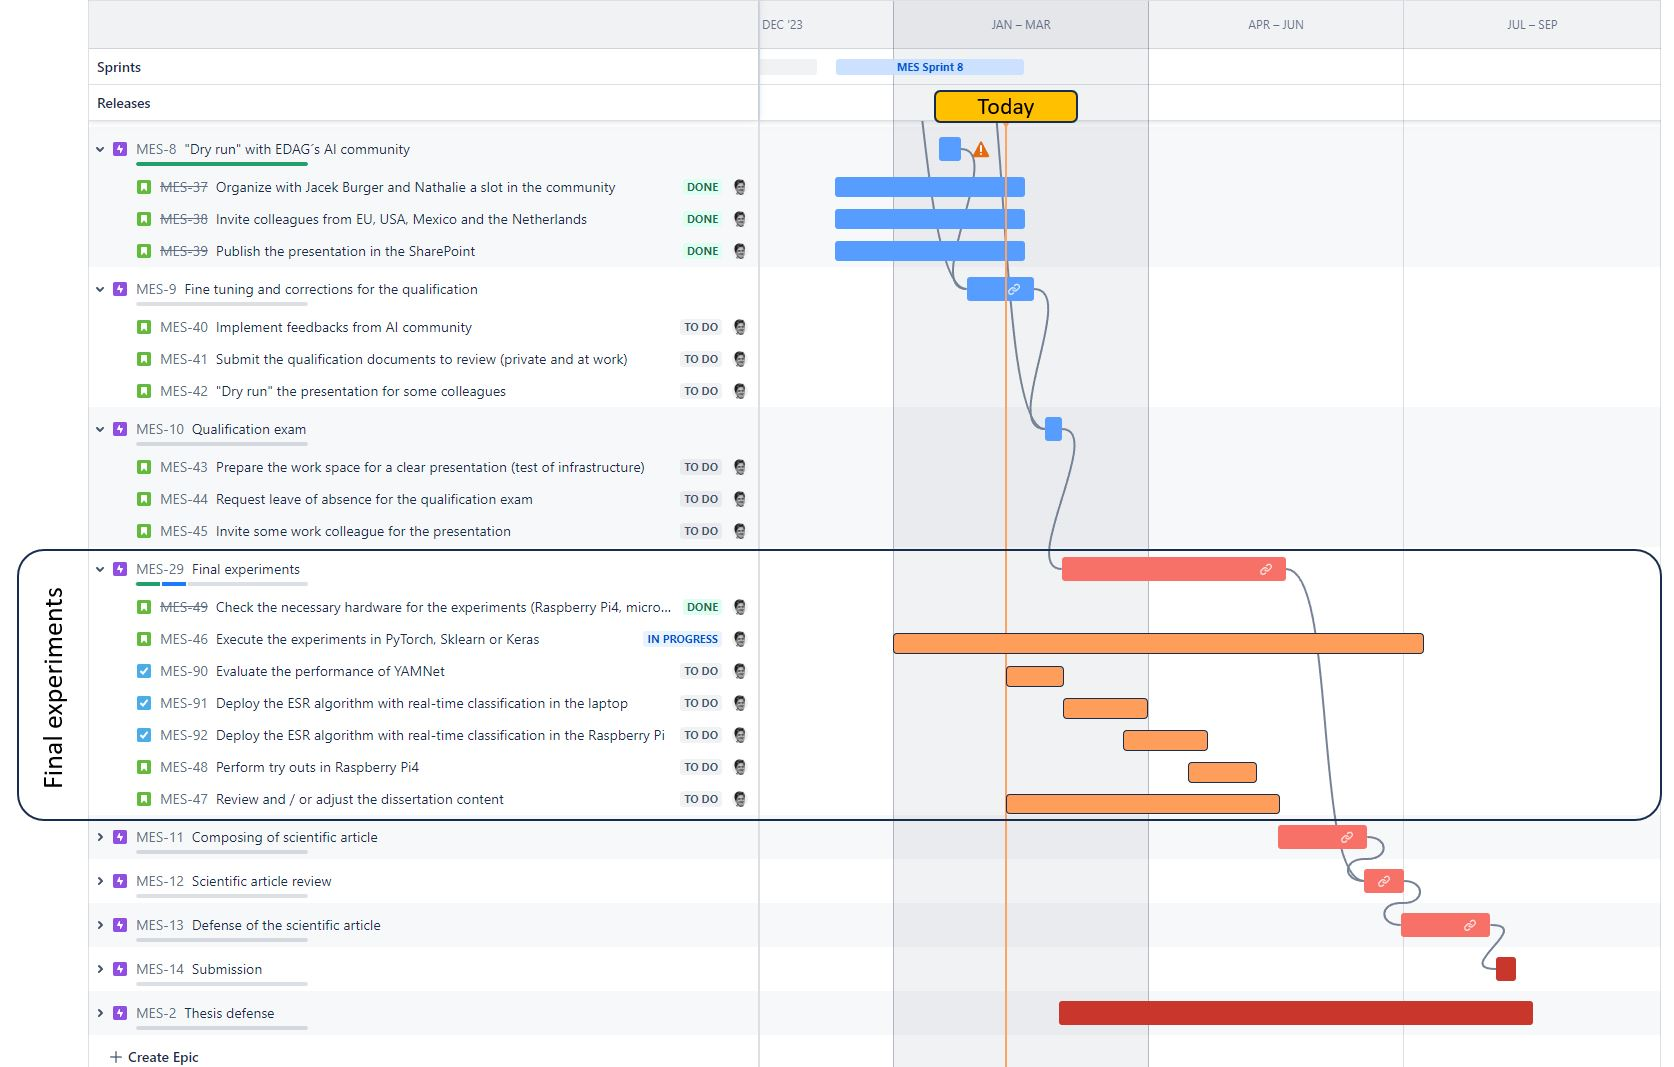
\includegraphics[width=1\textwidth]{resources/images/070-conclusion/Conclusion_roadmap_02.jpg}
        \smallcaption{Source: Author}
        \label{fig:conclusion_roadmap_2}
\end{figure}

\begin{figure}[htbp]
    \raggedright
        \caption{Roadmap, kanban and backlog.}
        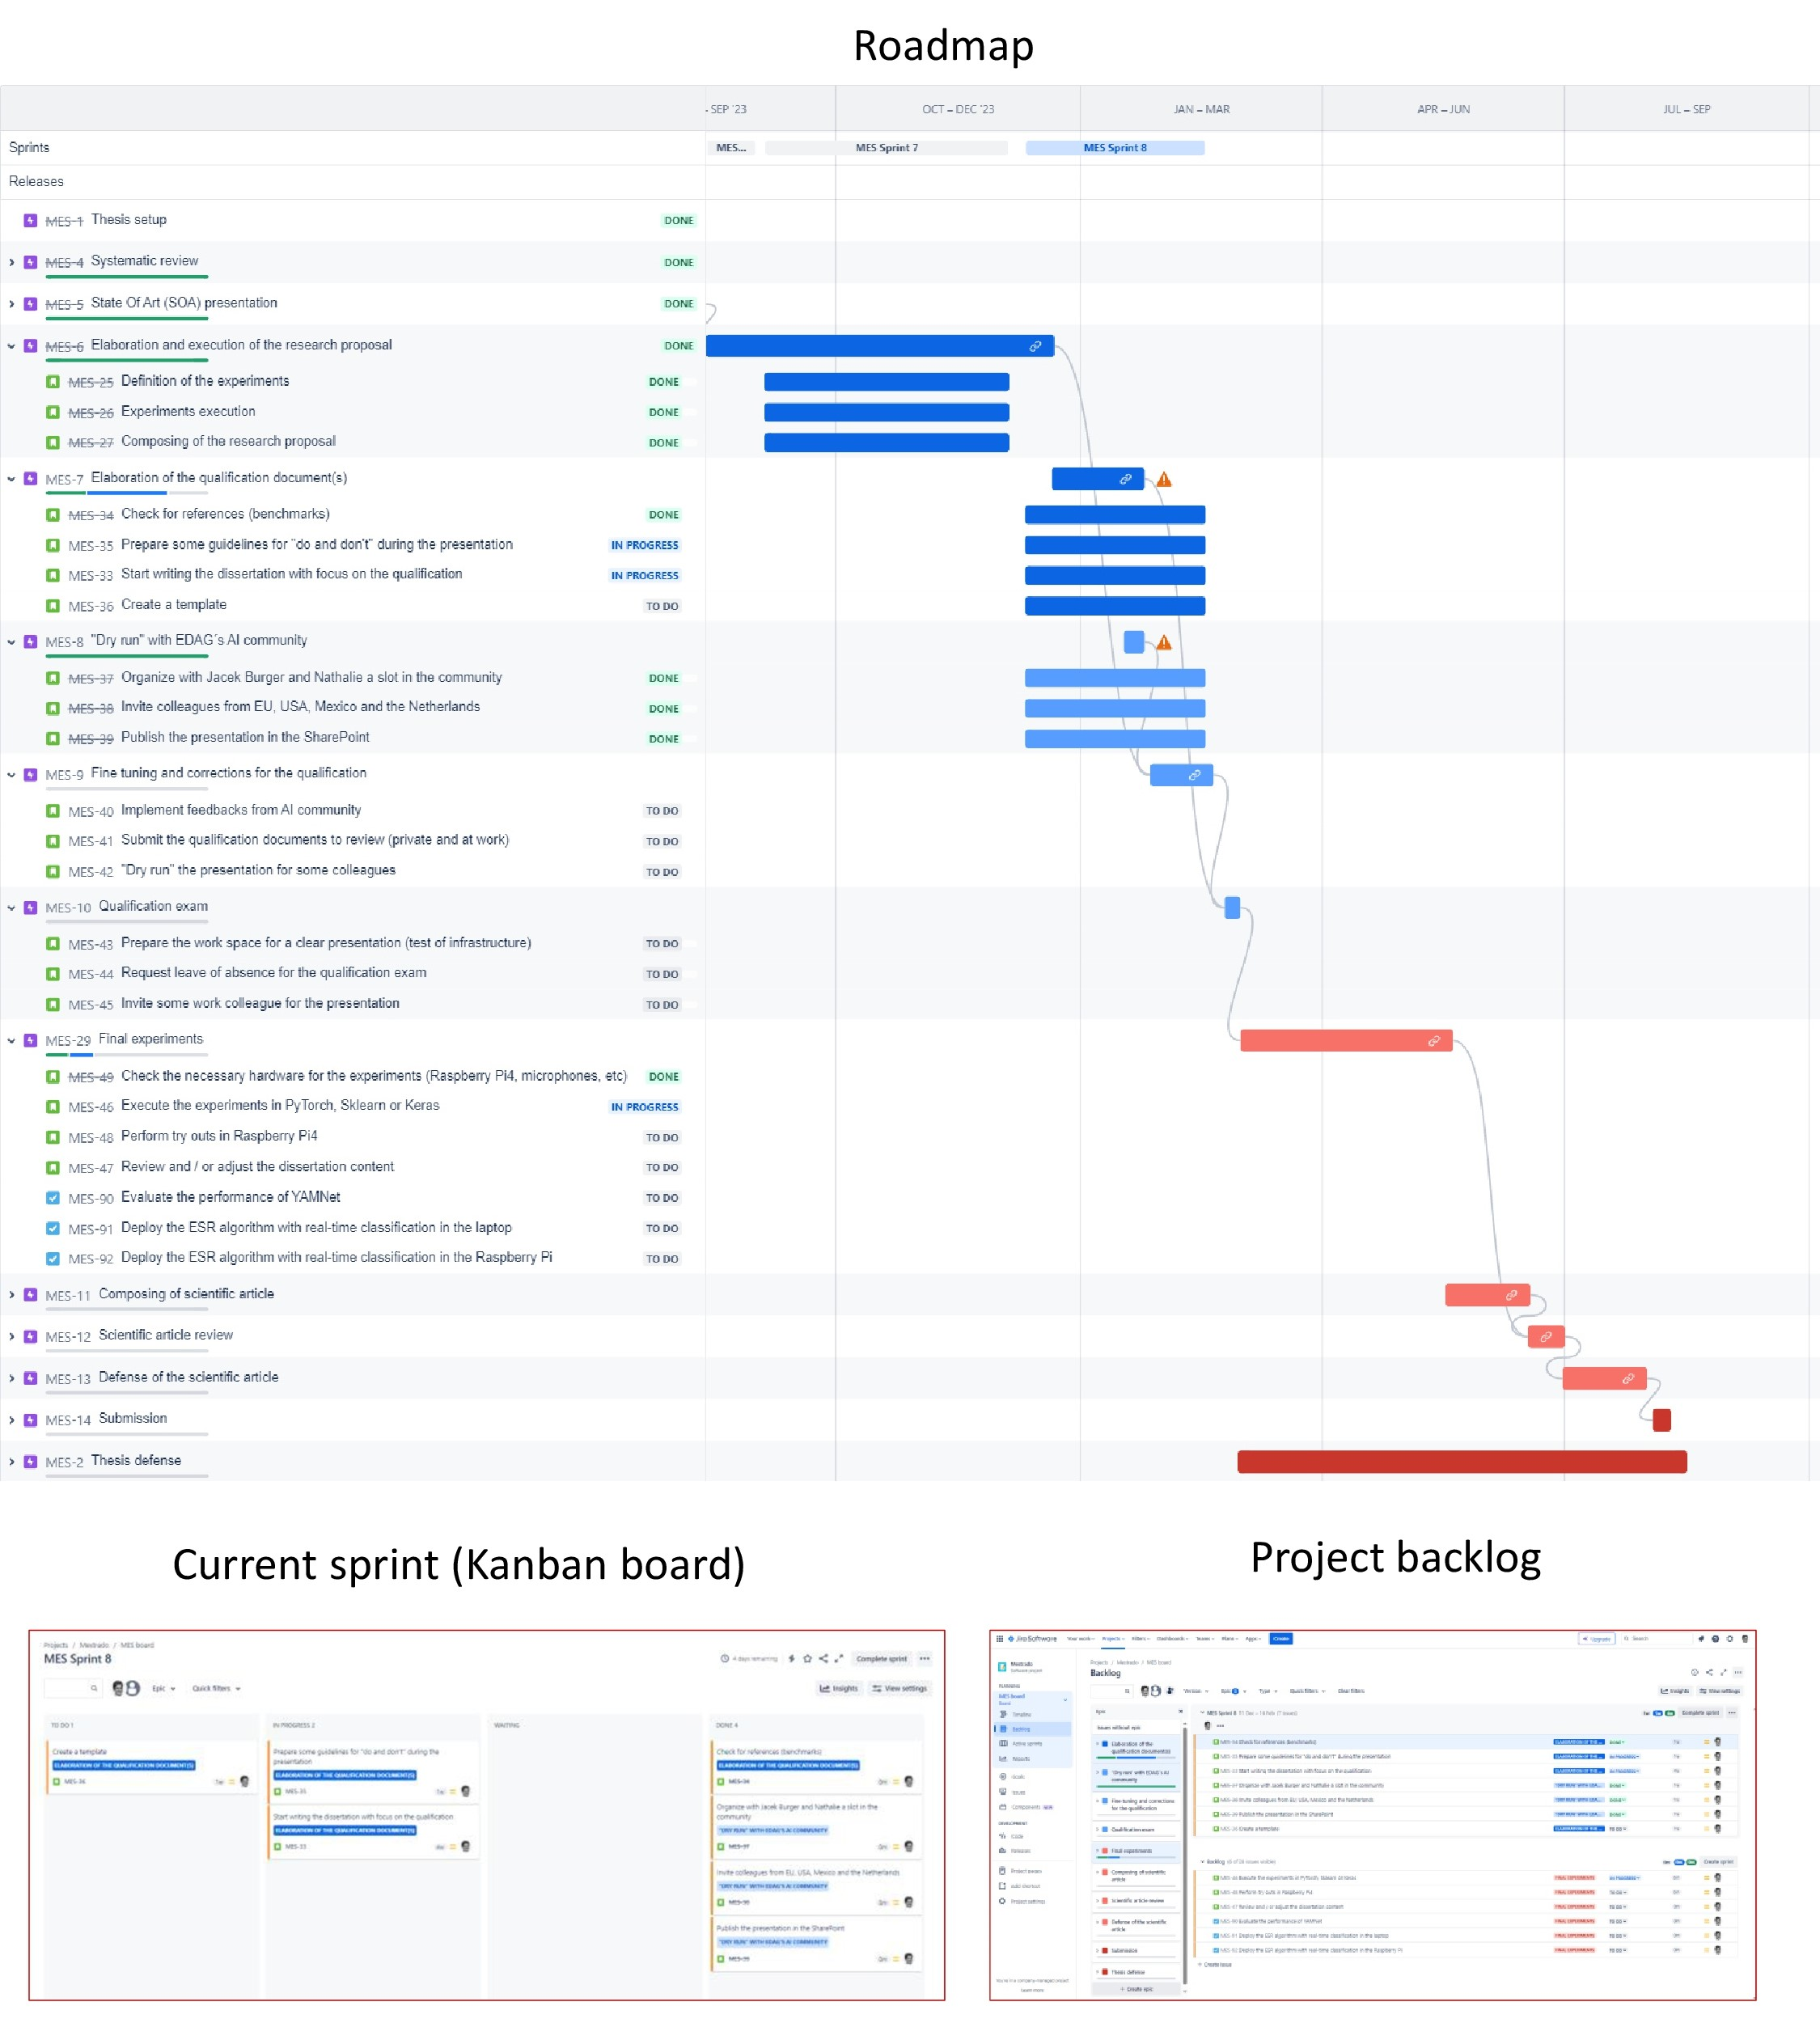
\includegraphics[width=1\textwidth]{resources/images/070-conclusion/Conclusion_roadmap_01.jpg}
        \smallcaption{Source: Author}
        \label{fig:conclusion_roadmap_1}
\end{figure}